\documentclass[12pt,a4paper]{article}
\usepackage[utf8]{inputenc}
\usepackage[T1]{fontenc}
\usepackage{amsmath}
\usepackage{amsfonts}
\usepackage[english]{babel}
\usepackage{amsthm}
\usepackage{mathrsfs}
\newtheorem*{remark}{Remark}

\usepackage{amssymb}
\usepackage{graphicx}
\DeclareMathOperator{\X}{\boldsymbol{X}}
\DeclareMathOperator{\Y}{\boldsymbol{Y}}

\begin{document}


\newpage

In the paper of "QLSD: Quantised Langevin stochastic dynamics for Bayesian federated learning", they do nothing but deal with the term
\begin{equation*}
	\int_{\mathrm{X}^{b}}\left\|\sum_{i=1}^{b} \mathscr{C}\left(F_{i}^{\star}\left(\theta, x^{(1, i)}\right), x^{(2, i)}\right)-\nabla U(\theta)\right\|^{2} \nu^{\otimes b}\left(\mathrm{~d} x^{(1: b)}\right),
\end{equation*}
$F^{\star}_i$ differs in different algorithms.
\newline
This is also true when we try to prove "Quantised underdamped langevin stochastic dynamics", corresponding to the red part in the above picture. $\nabla \tilde{f}$ will be replace by $\sum_{i=1}^{b} \mathscr{C}\left(F_{i}^{\star}\left(\theta, x^{(1, i)}\right), x^{(2, i)}\right),$ we can deal with this term like in "QLSD" without any difference(actually can be exact the same). The proof of theorem 4.3 is from "Underdamped Langevin MCMC: A non-asymptotic analysis"




\begin{figure}
	\centering
	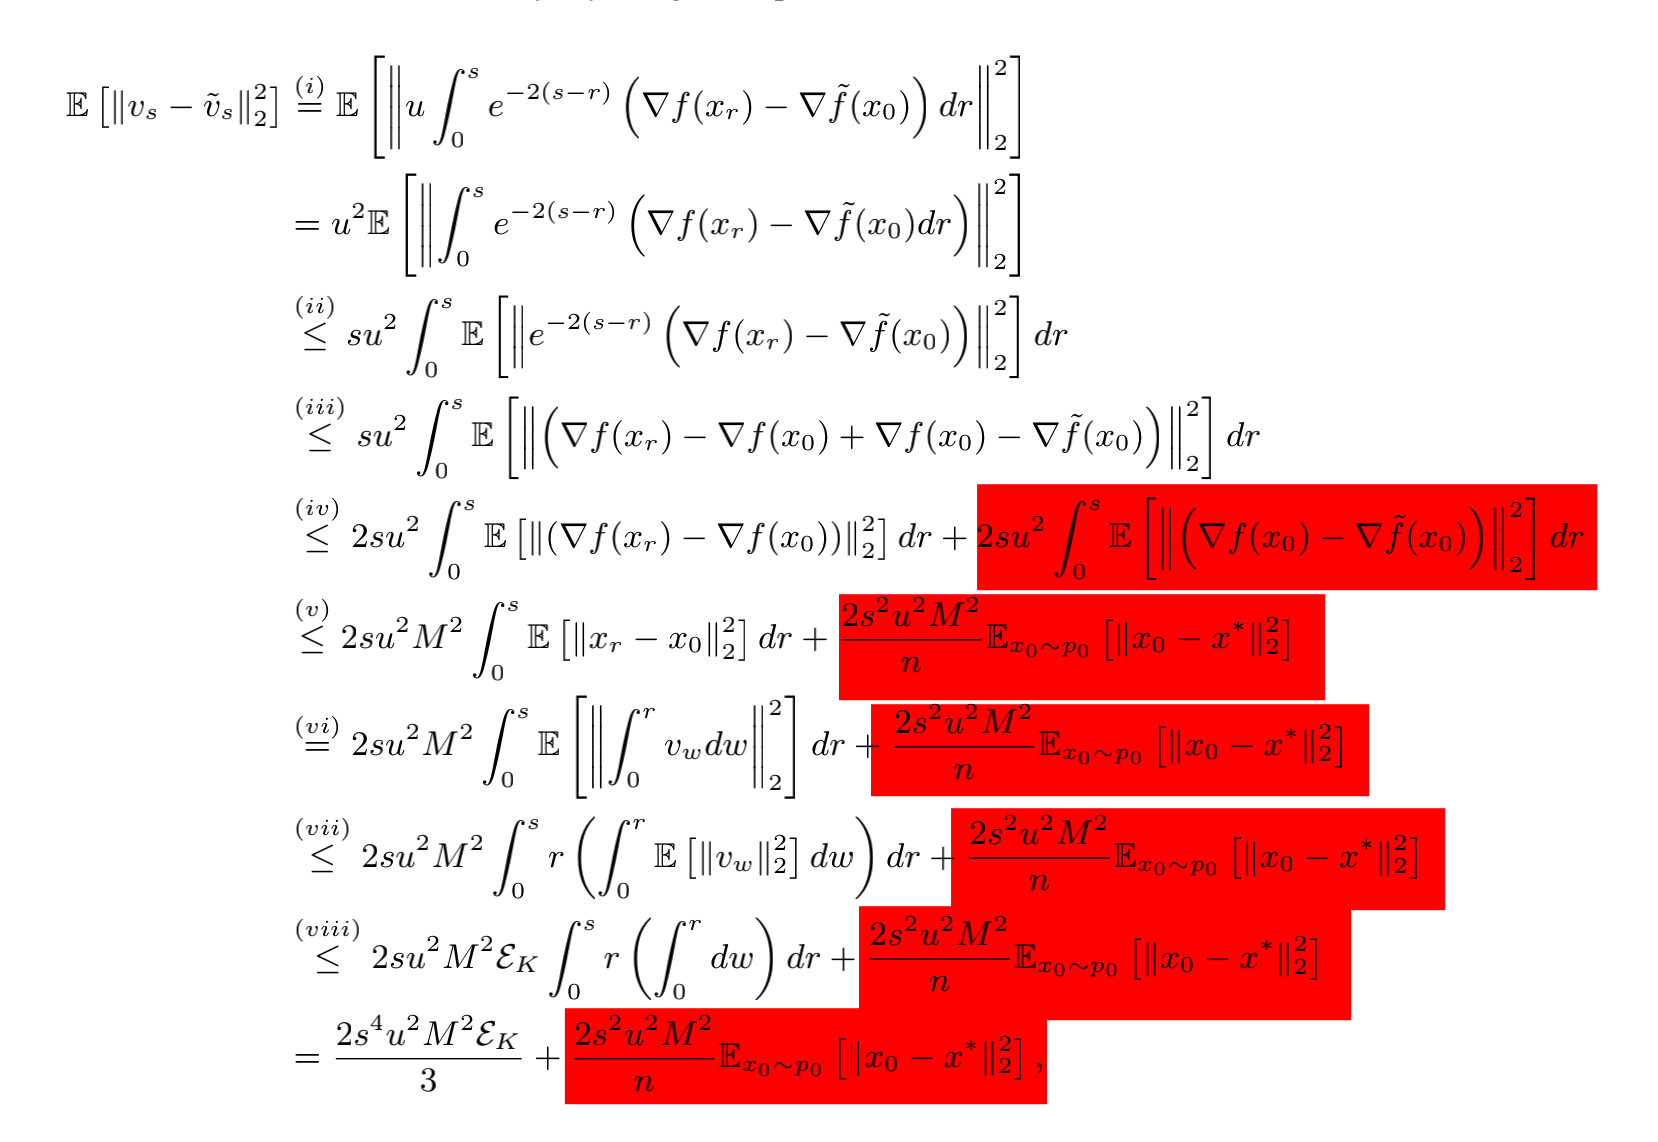
\includegraphics[width=0.7\linewidth]{jietu}
	\caption{copy from "On the Theory of Variance Reduction for Stochastic Gradient Monte Carlo " page 33.}
	\label{fig:jietu}
\end{figure}
















\end{document}